\documentclass[12pt, svgnames, titlepage]{report}

%%%%%%%%%%%%%%%%%%%%%%%%%%%%%%%%%%%%%%%%%%%%%%%%%%%%%%%%%%%%%%%%%%%%%%%%%%%%%%%%
%
% hyperref will allow of hyperlinks or making the table of contents links to the
% sections
%
%%%%%%%%%%%%%%%%%%%%%%%%%%%%%%%%%%%%%%%%%%%%%%%%%%%%%%%%%%%%%%%%%%%%%%%%%%%%%%%%
\usepackage{hyperref}
\hypersetup{
    colorlinks,
    citecolor=black,
    filecolor=black,
    linkcolor=black,
    urlcolor=black
}

%%%%%%%%%%%%%%%%%%%%%%%%%%%%%%%%%%%%%%%%%%%%%%%%%%%%%%%%%%%%%%%%%%%%%%%%%%%%%%%%
%
% fancyhdr allows for more elaborate header/footers on a page
%
%%%%%%%%%%%%%%%%%%%%%%%%%%%%%%%%%%%%%%%%%%%%%%%%%%%%%%%%%%%%%%%%%%%%%%%%%%%%%%%%
\usepackage{fancyhdr}
\pagestyle{fancyplain}

\usepackage{tikz}
\usetikzlibrary{arrows,backgrounds,positioning}

\author{Philip Tracton}
\date{\today}
\title{Block Diagrams}

\begin{document}

\maketitle
\newpage

\tableofcontents
\newpage
\listoffigures 
\newpage

\chapter{Simple Shapes and Colors}

\begin{figure}[h]
  \begin{tikzpicture}
    \draw (0,0) --(1,2);
  \end{tikzpicture}
  \caption{Simple Straight Line}
\end{figure}

\begin{figure}[h]
\begin{tikzpicture}[scale=3]
\draw (0,0) --(1,2) -- (2,3) -- (1,0);
\draw (0,3) -- (1.5,0.5);
\end{tikzpicture}
\caption{several lines scaled up}
\end{figure}

\begin{figure}[h]
  
\begin{tikzpicture}
    \draw [blue, fill=yellow] (0,0) rectangle (1.5,1);
    \draw [red, ultra thick] (3,0.5) circle [radius=0.5];;
    \draw [gray] (6,0) arc [radius=1, start angle=45, end angle= 120];
  \end{tikzpicture}
  \caption{Basic Shapes}
\end{figure}

\begin{figure}[h]
  \begin{tikzpicture}
    \draw [->] (1,1) -- (1,2);
    \draw [<-] (0, -0.5) -- (2,-0.5);
    \draw [|->] (0,-1) -- (2,-1);
    \draw [<->] (0,2) -- (0,0) -- (3,0);
  \end{tikzpicture}
  \caption{arrows}
\end{figure}

\begin{figure}[h]
  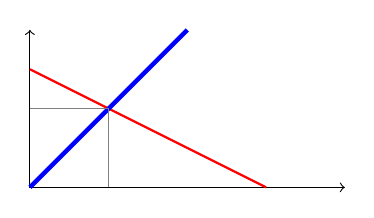
\begin{tikzpicture}
    \draw [<->] (0,2) -- (0,0) -- (4,0);
    \draw [red, thick] (0,1.5) -- (3,0);
    \draw [blue, ultra thick] (0,0) -- (2,2);
    \draw [help lines] (1,0) -- (1,1) -- (0,1);
  \end{tikzpicture}
  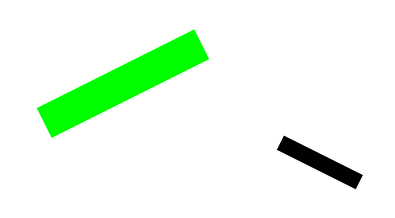
\begin{tikzpicture}
    \draw [green, line width=12] (1,1) -- (3,2);
    \draw [line width=0.2cm] (4,.75) -- (5,.25);
  \end{tikzpicture}     
  \caption{Line thickness}
\end{figure}

\newpage
\begin{figure}[h]
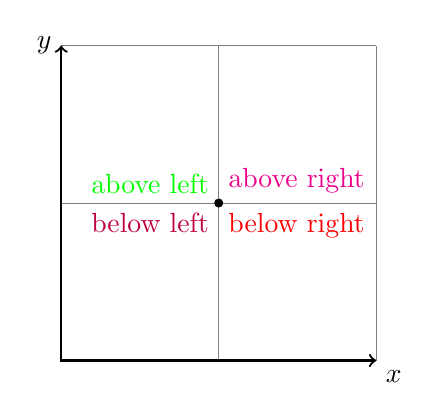
\begin{tikzpicture}[scale=2]
\draw[help lines] (0,0) grid (2,2);,
\draw [thick, <->] (0,2) -- (0,0) -- (2,0);
\draw[fill] (1,1) circle [radius=0.025];
\node [below right, red] at (1,1) {below right};
\node [above left, green] at (1,1) {above left};
\node [below left, purple] at (1,1) {below left};
\node [above right, magenta] at (1,1) {above right};
\node [left] at (0,2) {$y$};
\node [below right] at (2,0) {$x$};
\end{tikzpicture}
\caption{Text and pics}
\end{figure}


\begin{figure}[h]

\begin{tikzpicture}
\shade[top color=yellow,bottom color=black] (0,0) rectangle +(2,1);
\shade[left color=yellow,right color=black] (3,0) rectangle +(2,1);
\shadedraw[inner color=yellow,outer color=black,draw=yellow] (6,0) rectangle +(2,1);
\shade[ball color=green] (9,.5) circle (.5cm);
\end{tikzpicture}
\caption{Shading}
\end{figure}

\begin{figure}[h]

\begin{tikzpicture}[scale=2]
\tikz \foreach \x in {1,...,10}
\draw (\x,0) circle (0.4cm);
\end{tikzpicture}
\caption{For Loops}
\end{figure}

\begin{figure}[h]
\tikzstyle{place}=[circle,draw=blue!50,fill=blue!20,thick,
inner sep=0pt,minimum size=6mm]
\tikzstyle{transition}=[rectangle,draw=black!50,fill=black!20,thick,
inner sep=0pt,minimum size=4mm]
\begin{tikzpicture}
\node[place] (waiting) {};
\node[place] (critical) [below of=waiting] {};
\node[place] (semaphore) [below of=critical] {};
\node[transition] (leave critical) [right of=critical] {};
\node[transition] (enter critical) [left of=critical] {};
\node [red,above] at (semaphore.north) {$s\le 3$};
\draw [->] (enter critical.east) -- (critical.west);
\draw [->] (waiting.west) .. controls +(left:5mm) and +(up:5mm)
.. (enter critical.north);
\end{tikzpicture}
\caption{Styles}
\end{figure}
\chapter{Blocks}

\tikzstyle{MADSlaveIF}=[rectangle, draw=black, top color=yellow,bottom color=white, text height=2cm, text centered]
\tikzstyle{FIFO}=      [rectangle, draw=black, top color=blue,  bottom color=white, text height=1cm, text centered]

\begin{tikzpicture}[
    show background rectangle, 
    background rectangle/.style={fill=lightgray},
    box/.style={draw, font=\itshape}
]
\draw[help lines] (0,0) grid (16,10);
\node [MADSlaveIF] at (2,4) (MADSlaveInterface){MAD Slave Interface};
\node [FIFO] at (5,9) (WriteFIFO) {Write FIFO};
\node [FIFO] at (5,0) (ReadFIFO) {Read FIFO};
%\draw [->, ultra thick] (MADSlaveInterface.north) -- (WriteFIFO.west);
%\draw [->] (MADSlaveInterface.south) -- (ReadFIFO.north);
 \draw [<-, ultra thick] (MADSlaveInterface.south) -- (2,0) -- (ReadFIFO.west);
 \draw [->, ultra thick] (MADSlaveInterface.north) -- (2,9) -- (WriteFIFO.west);
%\node (MADSlaveInterface) at (2, 4)  [MADSlaveIF] (MAD Slave IF)[text height=6cm, text centered, top color=yellow,bottom color=white]{MAD Slave Interface};
%\shade[top color=yellow,bottom color=white] (0.5,1) rectangle +(1,6);
%\node [black] at (1,4) {MAD};
%\node [black] at (1,3.5) {Slave};
%\node [black] at (1,3) {IF};

\end{tikzpicture}
\end{document}